%definira klasu dokumenta 
\documentclass[12pt]{report} 

%prostor izmedu naredbi \documentclass i \begin{document} se zove uvod. U njemu se nalaze naredbe koje se odnose na cijeli dokument
	
	%osnovni LaTex ne može riješiti sve probleme, pa se koriste različiti paketi koji olakšavaju izradu željenog dokumenta
	\usepackage[utf8]{inputenc}
	%\usepackage[T1]{fontenc}
	\usepackage[croatian]{babel} 
	\usepackage{amssymb}
	\usepackage{amsmath}
	\usepackage{txfonts}
	\usepackage{mathdots}
	\usepackage{titlesec}
	\usepackage{array}
	\usepackage{lastpage}
	\usepackage{etoolbox}
	\usepackage{tabularray}
	\usepackage{color, colortbl}
	\usepackage{adjustbox}
	\usepackage{geometry}
	\usepackage[classicReIm]{kpfonts}
	\usepackage{hyperref}
	\usepackage{fancyhdr}
	
	\usepackage{float}
	\usepackage{setspace}
	\restylefloat{table}
	\usepackage{ragged2e}
	
	\usepackage{comment}
	
	\usepackage{listings}
	
	
	\patchcmd{\chapter}{\thispagestyle{plain}}{\thispagestyle{fancy}}{}{} %redefiniranje stila stranice u paketu fancyhdr
	
	%oblik naslova poglavlja
	\titleformat{\chapter}{\normalfont\huge\bfseries}{\thechapter.}{20pt}{\Huge}
	\titlespacing{\chapter}{0pt}{0pt}{40pt}
	
	
	\linespread{1.3} %razmak između redaka
	
	\geometry{a4paper, left=1in, top=1in,}  %oblik stranice
	
	\hypersetup{ colorlinks, citecolor=black, filecolor=black, linkcolor=black,	urlcolor=black }   %izgled poveznice
	
	
	%prored smanjen između redaka u nabrajanjima i popisima
	\newenvironment{packed_enum}{
		\begin{enumerate}
			\setlength{\itemsep}{0pt}
			\setlength{\parskip}{0pt}
			\setlength{\parsep}{0pt}
		}{\end{enumerate}}
	
	\newenvironment{packed_item}{
		\begin{itemize}
			\setlength{\itemsep}{0pt}
			\setlength{\parskip}{0pt}
			\setlength{\parsep}{0pt}
		}{\end{itemize}}
	
	
	
	
	%boja za privatni i udaljeni kljuc u tablicama
	\definecolor{LightBlue}{rgb}{0.9,0.9,1}
	\definecolor{LightGreen}{rgb}{0.9,1,0.9}
	
	%Promjena teksta za dugačke tablice
	\DefTblrTemplate{contfoot-text}{normal}{Nastavljeno na idućoj stranici}
	\SetTblrTemplate{contfoot-text}{normal}
	\DefTblrTemplate{conthead-text}{normal}{(Nastavljeno)}
	\SetTblrTemplate{conthead-text}{normal}
	\DefTblrTemplate{middlehead,lasthead}{normal}{Nastavljeno od prethodne stranice}
	\SetTblrTemplate{middlehead,lasthead}{normal}
	
	%podesavanje zaglavlja i podnožja
	
	\pagestyle{fancy}
	\lhead{Osnove statističkog programiranja}
	\rhead{}
	\cfoot{stranica \thepage/\pageref{LastPage}}
	\rfoot{\today}
	\renewcommand{\headrulewidth}{0.2pt}
	\renewcommand{\footrulewidth}{0.2pt}
	
	
	\begin{document} 
		
		
		
		\begin{titlepage}
			\begin{center}
				\vspace*{\stretch{1.0}} %u kombinaciji s ostalim \vspace naredbama definira razmak između redaka teksta
				\LARGE Osnove statističkog programiranja\\
				\large Ak. god. 2023./2024.\\
				
				\vspace*{\stretch{3.0}}
				
				\huge Neki naslov\\
				\Large Dokumentacija\\
				
				\vspace*{\stretch{12.0}}
				\normalsize
				Julijana Kolarec, Lucija Topolko\\
				
				
				\vspace*{\stretch{1.0}}
				siječanj 2024., Zagreb\\
				
				\vspace*{\stretch{4.0}}
				
				Nastavnik: \textit{prof.dr.sc. Damir Pintar}\\
				
			\end{center}
			
			
		\end{titlepage}
		
		
		\tableofcontents
		
		
		\definecolor{codegreen}{rgb}{0,0.6,0}
\definecolor{codegray}{rgb}{0.5,0.5,0.5}
\definecolor{codepurple}{rgb}{0.58,0,0.82}
\definecolor{backcolour}{rgb}{0.95,0.95,0.92}

\lstdefinestyle{mystyle}{
	backgroundcolor=\color{backcolour},   
	commentstyle=\color{codegreen},
	keywordstyle=\color{magenta},
	numberstyle=\tiny\color{codegray},
	stringstyle=\color{codepurple},
	basicstyle=\ttfamily\footnotesize,
	breakatwhitespace=false,         
	breaklines=true,                 
	captionpos=b,                    
	keepspaces=true,                 
	numbers=left,                    
	numbersep=5pt,                  
	showspaces=false,                
	showstringspaces=false,
	showtabs=false,                  
	tabsize=2
}

\lstset{style=mystyle}


\chapter{Prediktivni modeli primjenom strojnog učenja}

Kako bismo bolje razumjeli što film čini uspješnim ili neuspješnim, provele smo analizu dobivenog skupa podataka primjenom strojnog učenja. Cilj nam je bio razviti model koji može čim točnije predviđati uspjeh filma na temelju njegovih karakteristika.
\\
\section{Priprema podataka}
Iz dobivenih podataka izbacile smo retke kojima su nedostajali neki podaci. Takvih je redaka bilo 1261. Također, uklonile smo stupce koji su sadržavali jedinstvene ili skoro jedinstvene vrijednosti (\textit{movie\_title, movie\_imdb\_link, plot\_keywords, genres}). Još smo izbacile tekstualne stupce koji su bili prekorelirani s nekim numeričkim stupcem. Na primjer, \textit{actor\_1\_name} je prekoreliran s \textit{actor\_1\_facebook\_likes}. 

\lstinputlisting[language=R]{../R/001.R} 
Preostale nenumeričke stupce pretvorile smo u tip integer. 

\lstinputlisting[language=R]{../R/002.R}

Značajka koju predviđamo je \textit{imdb\_score}. To broj zaokružen na jednu decimalu, pa smo za bolje rezultate uspjeh filma podijelile u tri skupine: loš, osrednji i dobar, a stupac imdb\_score smo zbog prekoreliranosti uklonile. 

\lstinputlisting[language=R]{../R/003.R}

Graf \ref{fig:ml1} prikazuje omjer broja filmova po uspjehu. Filmova koji su ocijenjeni kao loši znatno je manje od ostalih. Točnije, loših je filmova 43, osrednjih 1981, a dobrih 1746.

\begin{figure}
	\centering
	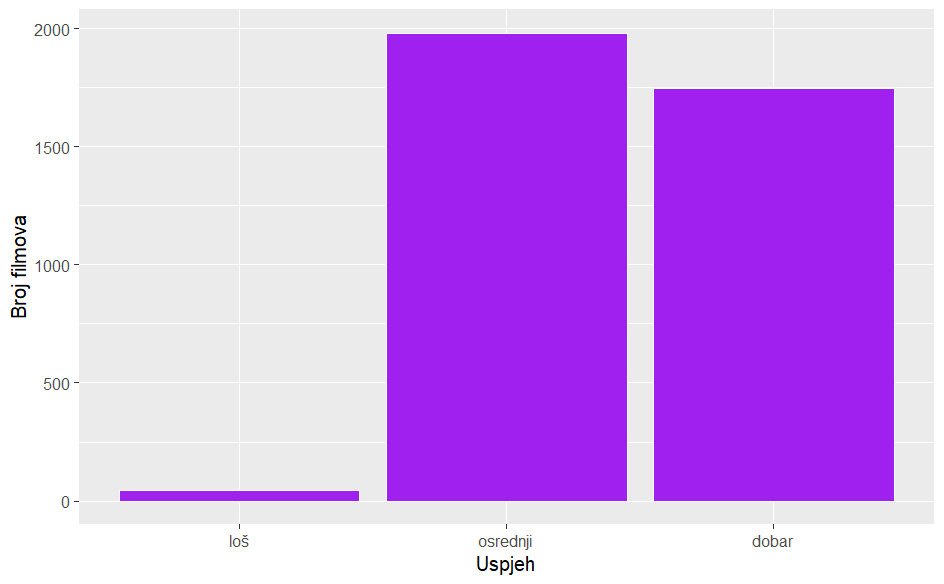
\includegraphics[width=15cm]{../figures/expl/001.png}
	\caption{Podjela filmova po uspjehu}
	\label{fig:ml1}
\end{figure}


\lstinputlisting[language=R]{../R/004.R}

\begin{center}
	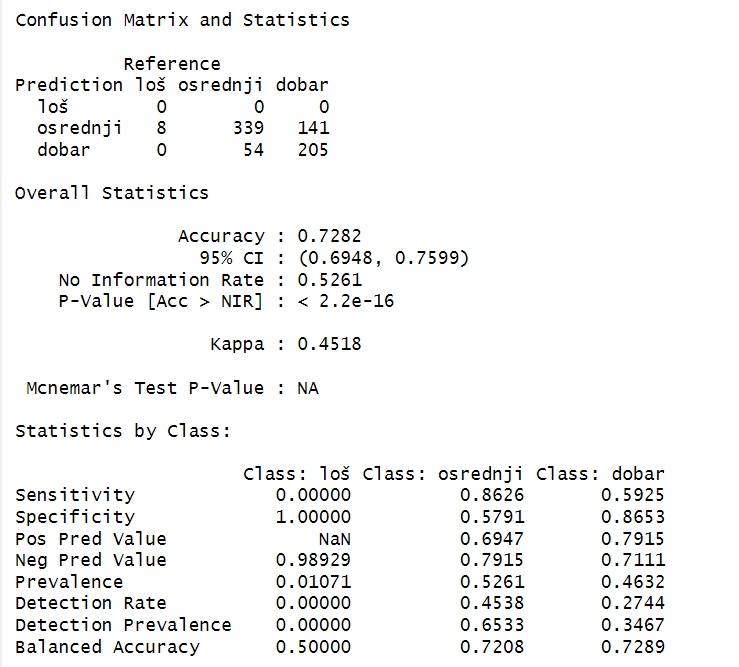
\includegraphics{../figures/expl/002.png}
\end{center}

\lstinputlisting[language=R]{../R/005.R}

\begin{center}
	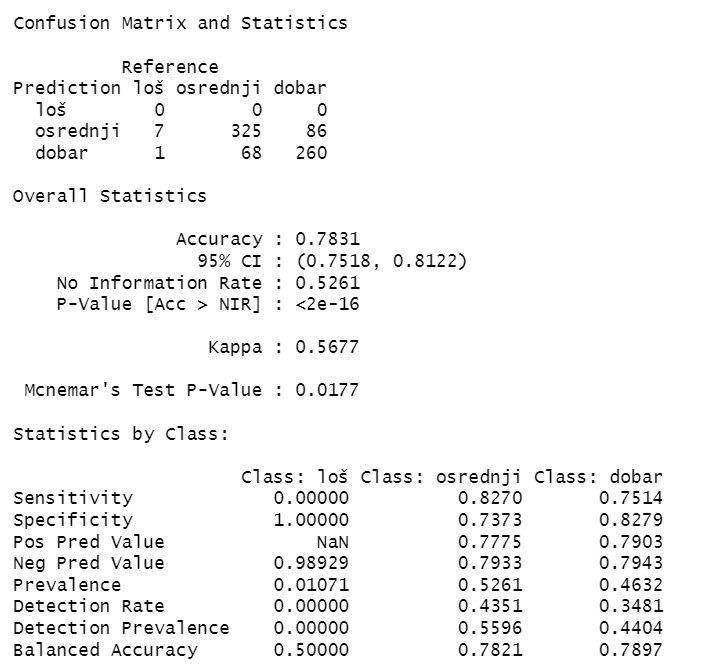
\includegraphics{../figures/expl/003.png}
\end{center}

\lstinputlisting[language=R]{../R/006.R}

\begin{center}
	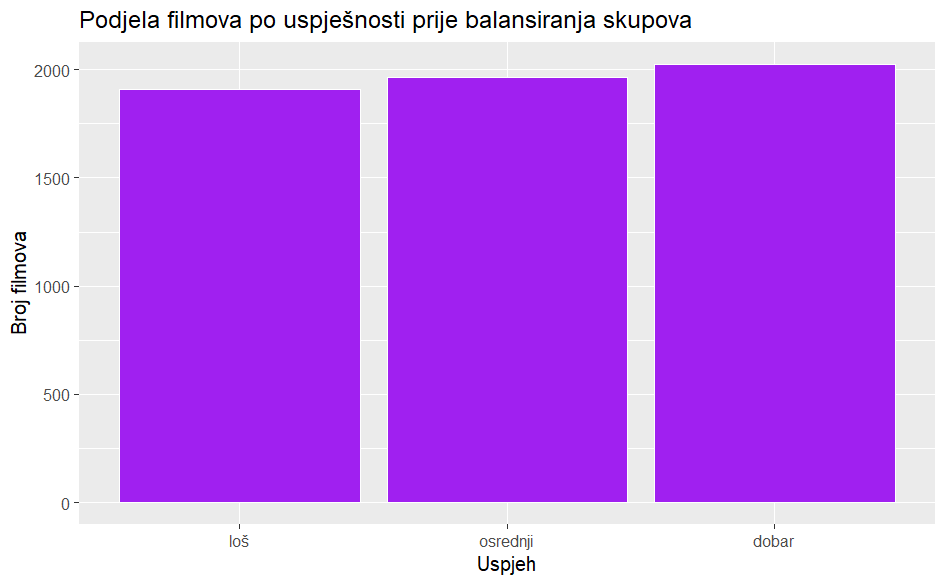
\includegraphics[width=15cm]{../figures/expl/004.png}
\end{center}

\begin{center}
	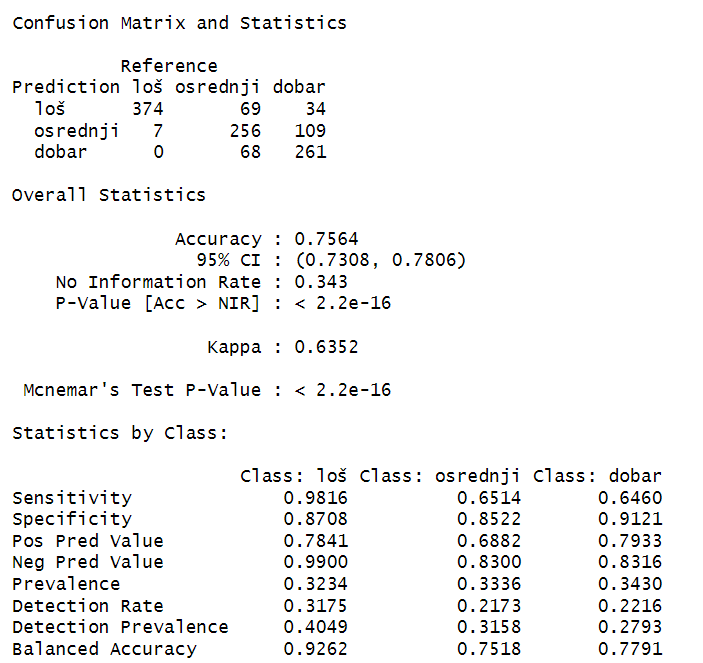
\includegraphics{../figures/expl/005.png}
\end{center}

\begin{center}
	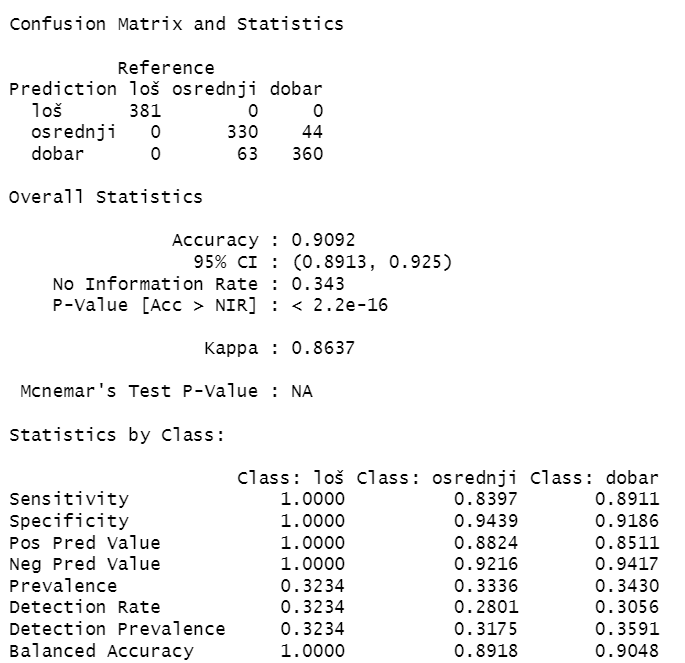
\includegraphics{../figures/expl/006.png}
\end{center}

\begin{center}
	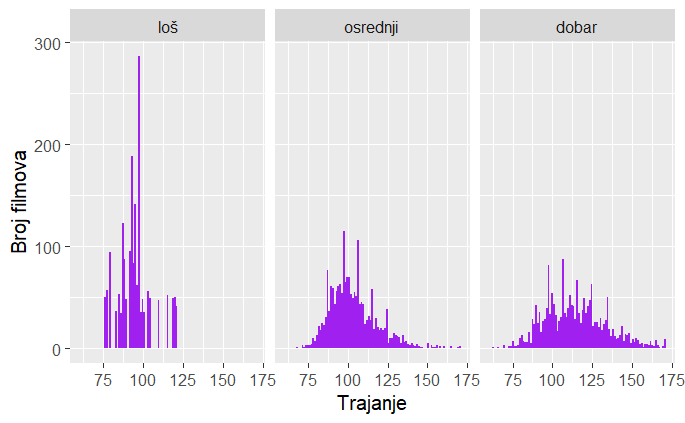
\includegraphics[width=15cm]{../figures/expl/007.png}
\end{center}

\begin{center}
	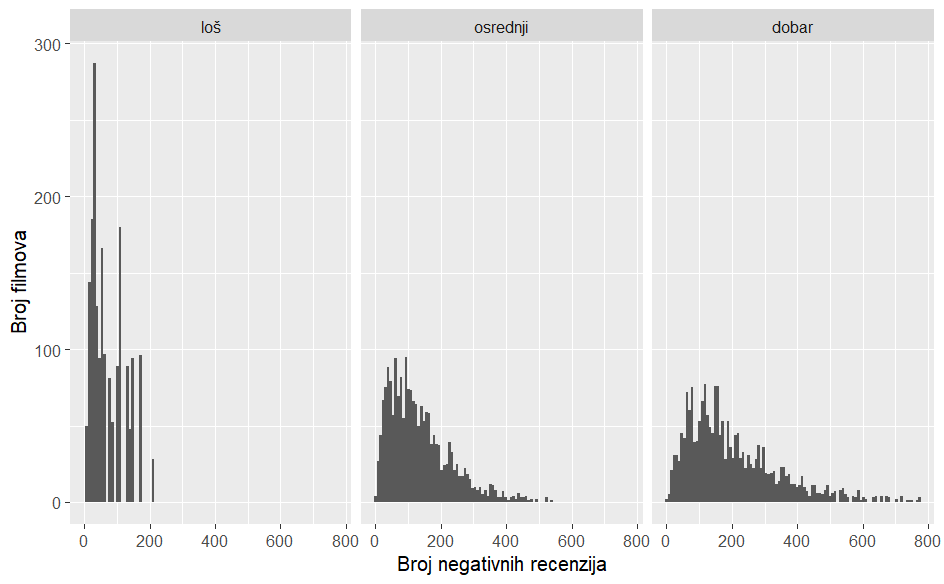
\includegraphics[width=15cm]{../figures/expl/008.png}
\end{center}


\eject
		
		
		\begingroup
		\renewcommand*\listfigurename{Indeks slika i dijagrama}
		%\renewcommand*\listtablename{Indeks tablica}
		%\let\clearpage\relax
		\listoffigures
		%\vspace{10mm}
		%\listoftables
		\endgroup
		\addcontentsline{toc}{chapter}{Indeks slika i dijagrama}
		
		
		
		\eject 
		
		
		
	\end{document} %naredbe i tekst nakon ove naredbe ne ulaze u izgrađen dokument 
	
